%%%%%%%%%%%%%%%%%%%%%%%%%%%%%%%%%%%%%%%%%%%%%%%%%%%%%%%%%%%%%%%%%%%%%%%%%%%%%%%%%%%%%%%%%%%%%%%%%%%%%%%%%%%%%%%%%%%%%%%%%%%%%%%%%%%%%%%%%%%%%%%%%%%%%%%%%%%%%%%%%%%%%%%%%%%%%%

\UC{Visualizzazione carrello}
\begin{figure}[H]
    \centering
    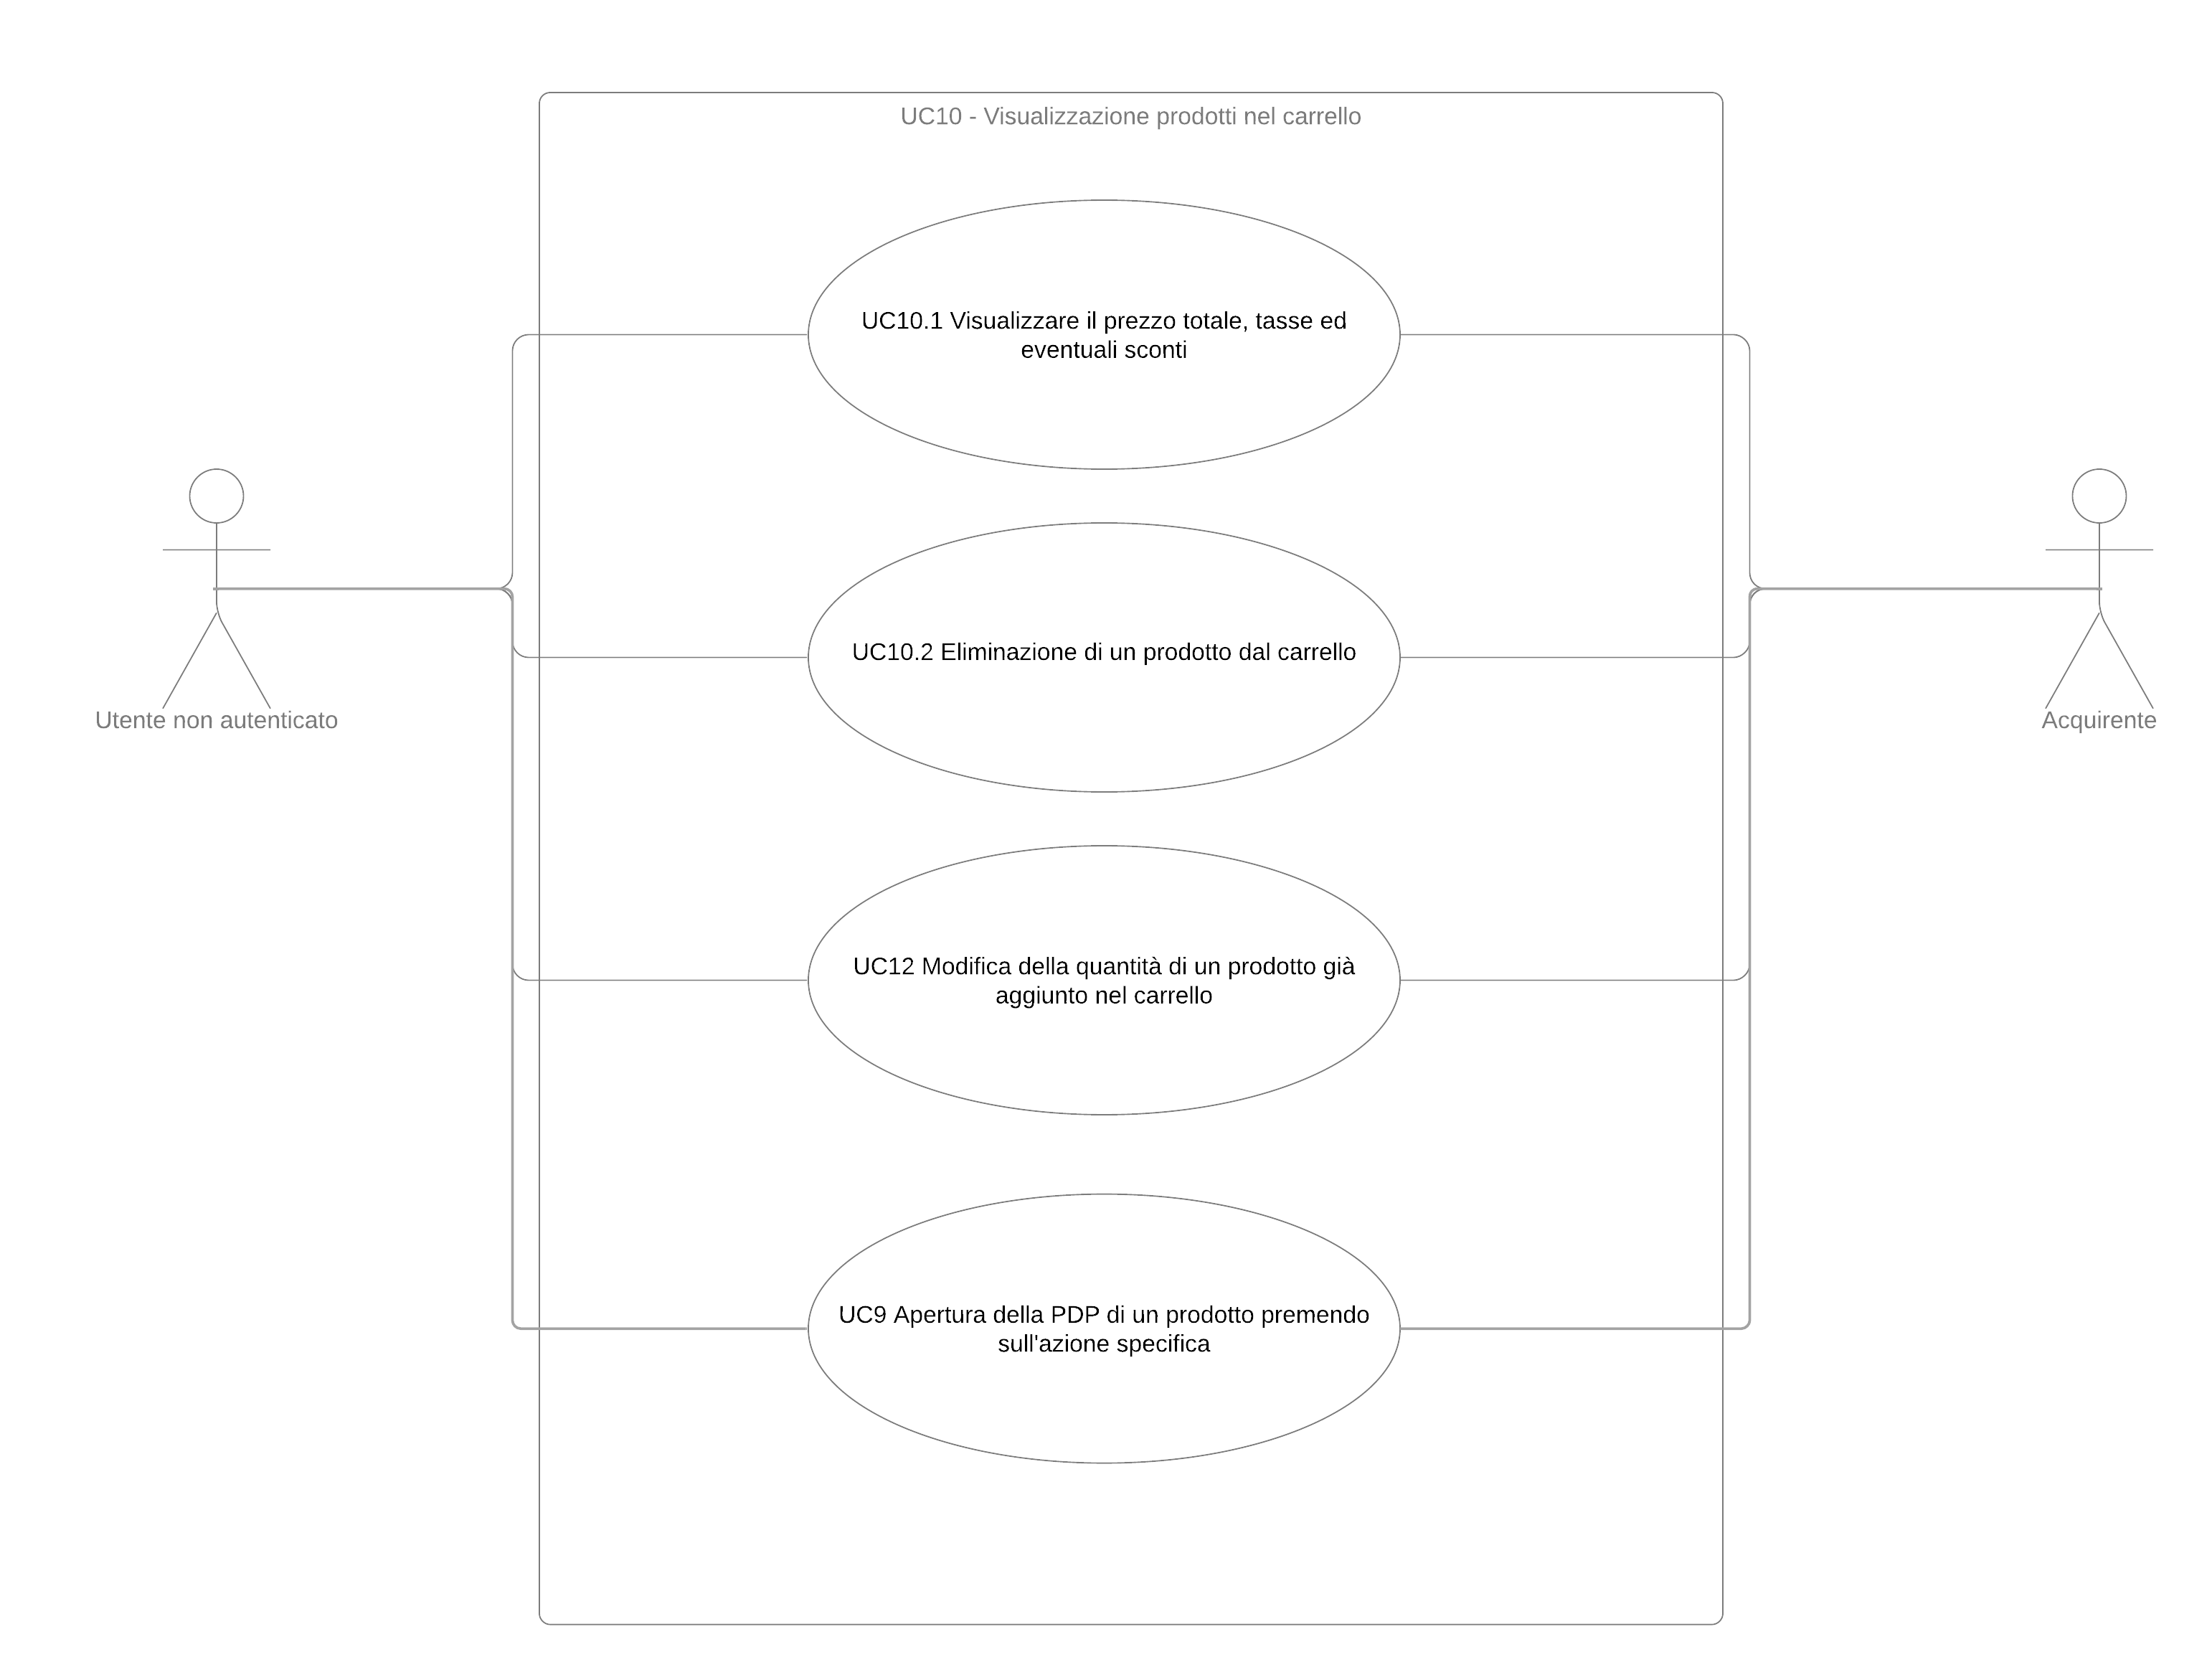
\includegraphics[width=\textwidth]{Immagini/DiagrammiUC/UC10VisualizzazioneProdottiNelCarrello.png}
    \caption{Diagramma di \actualUC: Visualizzazione prodotti nel carrello} 
    \label{fig:VisualizzazioneProdottiNelCarrello}
\end{figure}
L'utente vuole visualizzare il proprio carrello.
\begin{itemize}
    \item \textbf{Attori primari:} acquirente o utente non autenticato;
    \item \textbf{Precondizione:} l'attore si trova in una qualunque schermata della piattaforma;
    \item \textbf{Postcondizione:} l'attore visualizza il proprio carrello con l'elenco dei prodotti presenti;
    \item \textbf{Scenario principale:} l'attore seleziona la funzionalità per passare al carrello, da qui può:
    \begin{itemize}
        \item Visualizzare i prodotti presenti con il prezzo totale, tasse ed eventuali sconti;
        \item (UC) - Eliminare un prodotto dal carrello;
        \item (UC) - Modificare la quantità di un prodotto;
        \item (UC) - Aprire la PDP di un prodotto premendo sull'azione specifica;
        \item (UC) - Procedere al checkout.
    \end{itemize}
    \item \textbf{Scenari alternativi:} 
    \begin{enumerate}[label=\lett]
        \item se non ci sono prodotti all'interno del carrello, verrà visualizzato il messaggio "Carrello vuoto" e sarà data la possibilità all'attore di andare alla schermata principale per iniziare gli acquisti.
    \end{enumerate}
\end{itemize}

%%%%%%%%%%%%%%%%%%%%%%%%%%%%%%%%%%%%%%%%%%%%%%%%%%%%%%%%%%%%%%%%%%%%%%%%%%%%%%%%%%%%%%%%%%%%%%%%%%%%%%%%%%%%%%%%%%%%%%%%%%%%%%%%%%%%%%%%%%%%%%%%%%%%%%%%%%%%%%%%%%%%%%%%%%%%%%

\UC{Eliminazione di un prodotto dal carrello}
L'acquirente o l'utente non autenticato può eliminare un prodotto che ha inserito nel carrello.
\begin{itemize}
    \item \textbf{Attori Primari:} acquirente o utente non autenticato;
    \item \textbf{Precondizione:} l'attore è nella pagina del carrello e ha inserito almeno un prodotto;
    \item \textbf{Postcondizione:} l'attore ha rimosso totalmente il prodotto dal carrello;
    \item \textbf{Scenario Principale:} l'attore non vuole più ordinare un prodotto che ha aggiunto nel carrello e, per farlo, svolge le seguenti operazioni:
    \begin{itemize}
        \item clicca sull'azione di eliminazione del prodotto dal carrello;
        \item il prodotto viene rimosso dal carrello.
    \end{itemize}
\end{itemize}

%%%%%%%%%%%%%%%%%%%%%%%%%%%%%%%%%%%%%%%%%%%%%%%%%%%%%%%%%%%%%%%%%%%%%%%%%%%%%%%%%%%%%%%%%%%%%%%%%%%%%%%%%%%%%%%%%%%%%%%%%%%%%%%%%%%%%%%%%%%%%%%%%%%%%%%%%%%%%%%%%%%%%%%%%%%%%%

% \UC{Aggiunta del prodotto al carrello}
% \begin{figure}[H]
%     \centering
%     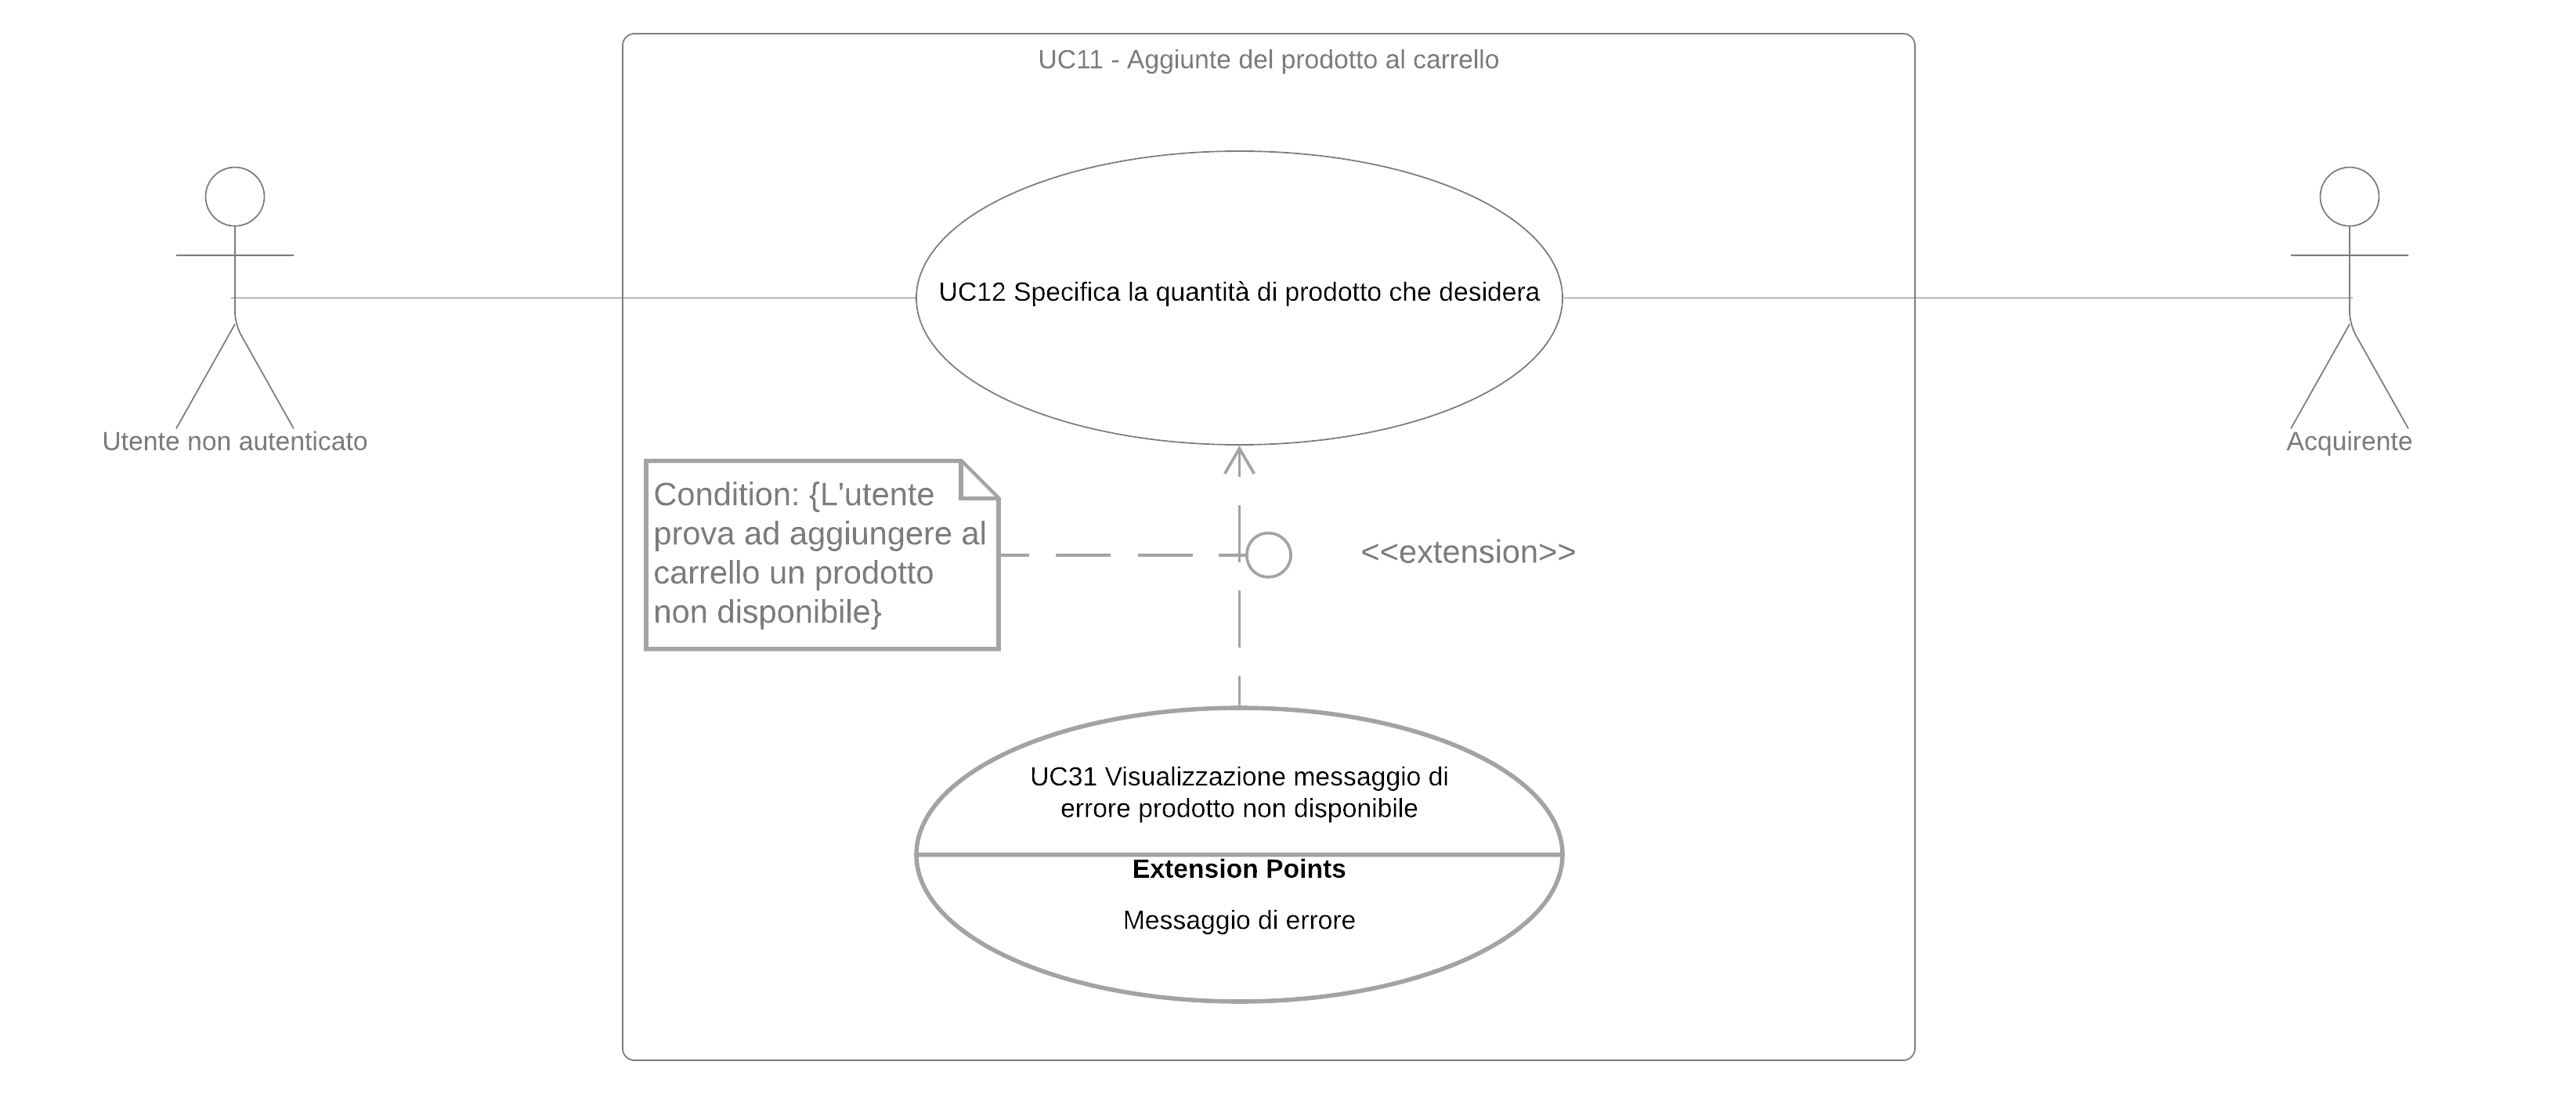
\includegraphics[width=\textwidth]{Immagini/DiagrammiUC/UC11AggiuntaProdottoAlCarrello.png}
%     \caption{Diagramma di \actualUC: Aggiunta del prodotto al carrello}
%     \label{fig:Checkout}
% \end{figure}

% L'utente non autenticato o l'acquirente può aggiungere al carrello i prodotti.
% \begin{itemize}
%     \item \textbf{Attori Primari:} Acquirente; Utente non autenticato
%     \item \textbf{Precondizione:} L'attore richiede di aggiungere una certa quantità del prodotto al carrello. 
%     \item \textbf{Postcondizione:} L'attore ha aggiunto la quantità desiderata di prodotto al carrello.
%     \item \textbf{Scenario Principale:} 
%     \begin{itemize}
%         \item (UC12) - Specifica la quantità di prodotto che desidera.
%         \item L'attore aggiunge il prodotto al carrello.
%         \item Il suo carrello personale viene aggiornato con il nuovo prodotto nella quantità indicata.
%     \end{itemize}
% \end{itemize}

%%%%%%%%%%%%%%%%%%%%%%%%%%%%%%%%%%%%%%%%%%%%%%%%%%%%%%%%%%%%%%%%%%%%%%%%%%%%%%%%%%%%%%%%%%%%%%%%%%%%%%%%%%%%%%%%%%%%%%%%%%%%%%%%%%%%%%%%%%%%%%%%%%%%%%%%%%%%%%%%%%%%%%%%%%%%%%

\UC{Modifica della quantità di un prodotto nel carrello}
L'acquirente o l'utente non autenticato modifica la quantità del prodotto già nel carrello.
\begin{itemize}
    \item \textbf{Attori primari:} acquirente o utente non autenticato;
    \item \textbf{Precondizione:} l'attore ha inserito un prodotto nel carrello e desidera modificarne la sua quantità;
    \item \textbf{Postcondizione:} la quantità del prodotto inserito nel carrello è aggiornata;
    \item \textbf{Scenario Principale:}
        \begin{itemize}
            \item l'attore aumenta o diminuisce la quantità tra 1 e la disponibilità massima di prodotto;
            \item la nuova quantità di prodotto sarà quella fornita.
        \end{itemize}
\end{itemize}

%%%%%%%%%%%%%%%%%%%%%%%%%%%%%%%%%%%%%%%%%%%%%%%%%%%%%%%%%%%%%%%%%%%%%%%%%%%%%%%%%%%%%%%%%%%%%%%%%%%%%%%%%%%%%%%%%%%%%%%%%%%%%%%%%%%%%%%%%%%%%%%%%%%%%%%%%%%%%%%%%%%%%%%%%%%%%%

\UC{Visualizzazione riepilogo ordini in gestione}
Il venditore vuole vedere gli ordini gestiti o da gestire.
\begin{itemize}
    \item \textbf{Attori primari:} venditore;
    \item \textbf{Precondizione:} il venditore da qualsiasi schermata in cui si trovi vuole visualizzare gli ordini da gestire/gestiti;
    \item \textbf{Postcondizione:} Viene aperta la pagina di riepilogo ordini;
    \item \textbf{Scenario principale:}
    \begin{itemize}
        \item L'attore seleziona la funzione per visualizzare il riepilogo degli ordini in gestione;
        \item Viene indirizzato alla schermata con tutti gli ordini a suo carico, per ogni ordine sono indicati i prodotti acquistati, la quantità e l'indirizzo di spedizione.
    \end{itemize}
\end{itemize}
